% Editable report section: Algorithm Design and Data Structures
\section{Algorithm Design and Data Structures}
\label{sec:3}

The architecture separates construction, validation and presentation so that each can be checked independently. Geometry, event management and the AVL tree use the Python standard library. Matplotlib draws the static diagrams and point-entry interface. An offline Canvas viewer presents recorded states from the same sweep engine. SciPy is installed separately for reference validation and is not imported by the construction core. The validators live under tests and outside the construction pipeline, so their nearest-site scans cannot supply the cells they are meant to check.

\begin{figure}[!htbp]
\centering
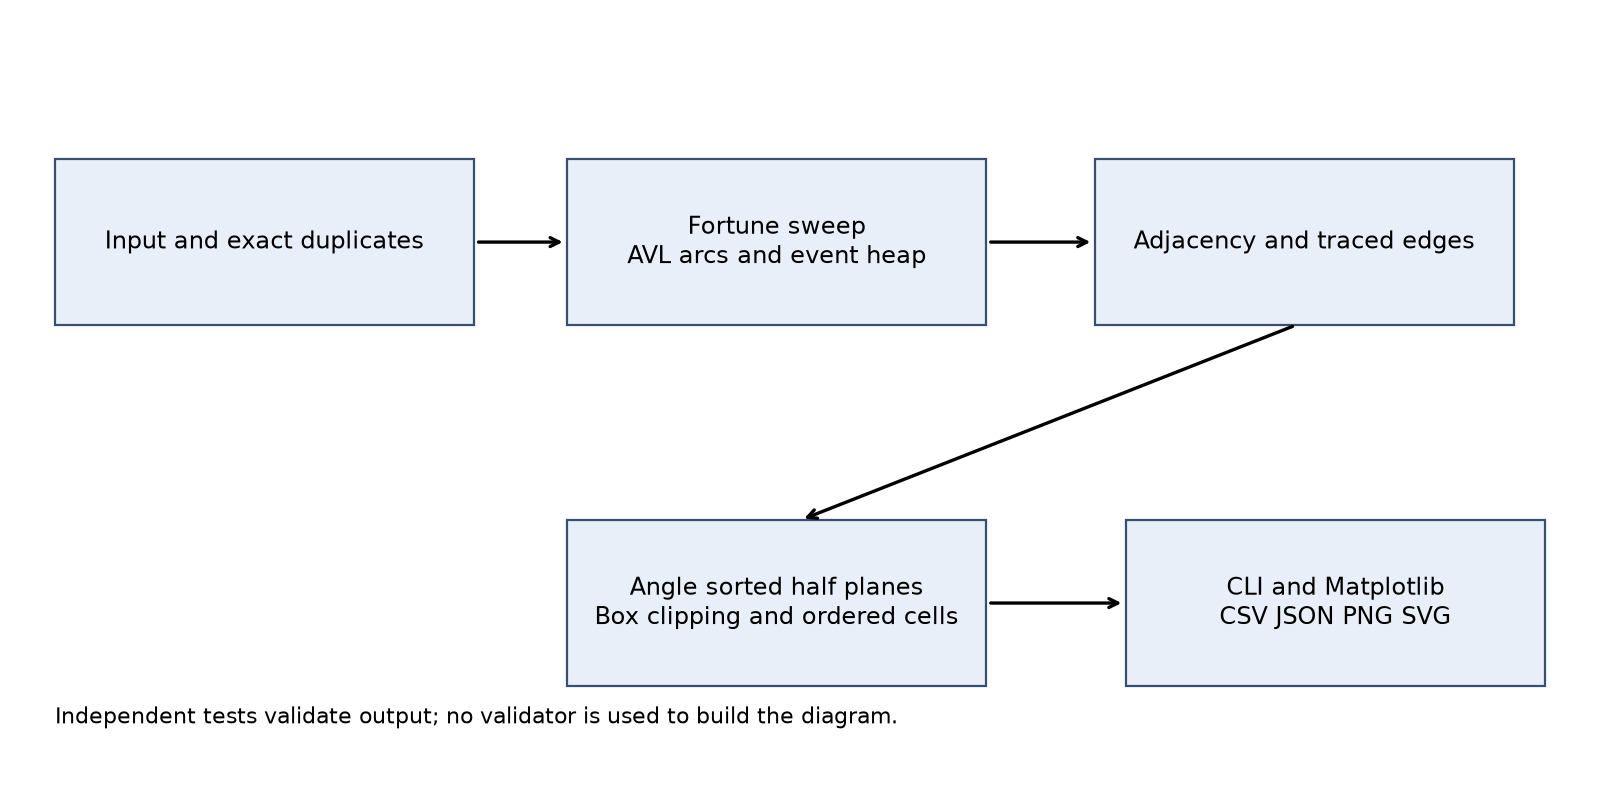
\includegraphics[width=1.0\linewidth,height=0.40\textheight,keepaspectratio]{architecture.png}
\caption{Construction pipeline and independent output validation.}
\label{fig:3}
\end{figure}

\begin{table}[!htbp]
\centering
\caption{Module responsibilities in the implemented system.}
\label{tab:2}
\begin{tabularx}{\linewidth}{@{}p{0.40\linewidth}X@{}}
\toprule
\textbf{Component} & \textbf{Main responsibility} \\
\midrule
\path{geometry.py} and \path{frame.py} & Filtered predicates, constructions and an exact uniform coordinate transform \\
\path{beachline.py} & Stable arc identities and AVL order \\
\path{events.py} and \path{circle.py} & Priority queue and candidate circle events \\
\path{sweep.py} & Site splits, arc removal, vertices and traced edges \\
\path{clipping.py} and \path{diagram.py} & Neighbour constraints and ordered clipped cells \\
\path{io.py}, \path{cli.py}, \path{interactive.py}, \path{visualize.py} & Inputs, exports, batch display and Delaunay overlay \\
\path{replay.py}, \path{replay_state.py}, \path{replay_canvas.py} & Event stepping, bounded checkpoints and browser replay \\
\bottomrule
\end{tabularx}
\end{table}

Each arc stores tree links, predecessor/successor links, height, site identifier, live state and a generation counter. A site can own several arcs, so its identifier cannot serve as a unique arc identity. Deletion transplants the successor node rather than copying its payload. This preserves queued references to the other arc objects.

\subsection{Invariants, Complexity and Numerical Policy}

The beach-line invariant is that the tree's in-order traversal equals the live left-to-right arc sequence, with consistent adjacent links. Search compares a query \(x\) against the node's current left and right breakpoints. AVL rotations preserve sequence order. Tests validate parent pointers, stored heights, balance and neighbour links after each randomized update.

The queue invariant is that the next valid event has the greatest remaining sweep height. The first heap key compares descending event heights. Ordinary separated heights use doubles; close circle heights are compared as exact rational-plus-square-root expressions. Event kind, horizontal position and a monotonically increasing serial number break equal-height ties. Site events precede circle events at equal height. A circle is valid only while its arc is alive and its stored generation equals the arc's current generation. Rescheduling increments that generation; stale entries are discarded when popped.

Each structural update creates only a constant number of candidates. AVL updates and heap operations cost $O(\log n)$, giving the intended $O(n \log n)$ sweep with $O(n)$ records. Traced adjacencies form a planar graph; hull order distinguishes true rays from zero-length cocircular diagonals. For cell degree \(k\), final intersection sorts \(k\) neighbour constraints plus four box constraints and uses a deque. Its cost is $O(k \log k)$; summing degrees in the planar graph preserves an $O(n \log n)$ overall target. It does not compare each cell with every site.

For neighbouring sites \(p_i\) and \(p_j\), the half-plane retained for \(p_i\) is equivalently
\begin{equation}
  2(p_j-p_i)\cdot q
  \leq \lVert p_j\rVert_2^2-\lVert p_i\rVert_2^2.
  \label{eq:halfplane}
\end{equation}
The implementation rescales this constraint and intersects only constraints generated by sweep neighbours.

\begin{table}[!htbp]
\centering
\caption{Numerical policies and their scope.}
\label{tab:3}
\begin{tabularx}{\linewidth}{@{}p{0.34\linewidth}X@{}}
\toprule
\textbf{Numerical operation} & \textbf{Current policy} \\
\midrule
Construction frame & Power-of-two scale with an exact translation or zero origin \\
Orientation cancellation & Filtered double sign, exact rational fallback \\
Close breakpoint searches & Exact rational comparison with the selected quadratic root \\
Ill-conditioned centre & Closest-pair origin and Decimal cancellation fallbacks \\
Close event heights & Exact comparison of rational radical expressions \\
Near-parallel half-planes & Rebuild coefficients from defining sites in Decimal \\
Clipping membership & Exact rational signs for uncertain corner tests \\
Repeated circle vertices & Exact input-circle identity, not coordinate rounding \\
\bottomrule
\end{tabularx}
\end{table}

These policies improved the tested cases, but they do not certify topology for every floating-point input. Coordinate construction still uses fixed 80-digit fallbacks and rounded output. A transform that loses subnormal coordinate bits is rejected explicitly. The complexity analysis counts arithmetic operations; the cost of exact rational fallbacks also depends on operand size. A fully certified geometry kernel would require stronger guarantees \cite{shewchuk1997}.
